\chapter{Comparison and Evaluation}
\label{sec:comparison_and_evaluation}

In this section, we compare the fuzzy tuning technique with other tuning techniques present in AutoPas an evaluate its performance.

To measure the performance of the tuning strategy, we also use the scenarios present in \gls{mdflexible}. The benchmarks are run on the CoolMuc-2 cluster at the Leibniz Supercomputing Centre in Garching \todo{add specs}.



\subsection{Exploding Liquid Benchmark}

The exploding liquid benchmark simulates a high-density liquid that quickly expands outwards as the simulation progresses. As the data of this scenario was included in the training data, we expect the fuzzy tuning technique to perform well. The benchmark is repeated with 1, 12, 24 and 28 threads, but for brevity, we only include the results for 1 and 28 threads as the other results are very similar. Every scenario is run with all available tuning strategies in AutoPas.

We use the \texttt{timeSpentCalculatingForces} metric to evaluate the performance of the tuning strategies as it gives a good indication of the performance of the configuration. The resulting timings are shown in \ref{fig:explodingLiquid1Benchmark_1thread} and \ref{fig:explodingLiquid1Benchmark_28thread} for 1 and 28 threads, respectively.

As timing data is prone to noise, we also include a heatmap of the selected configurations in \ref{fig:explodingLiquid1Heatmap_1thread} and \ref{fig:explodingLiquid1Heatmap_28thread} respectively. We can see that every tuning strategy selects a similar configuration most of the time. There are also some bigger deviations in both fuzzy tuning strategies, but we can see from the associated timings that these configurations are also very performant and do not significantly harm the total performance.

The last plot in \ref{fig:explodingLiquid1TotalTime_1thread} and \ref{fig:explodingLiquid1TotalTime_28thread} shows the total time spent calculating the forces for each tuning strategy. In every benchmark the fuzzy tuning strategies performed the best, with the individual tuning approach performed slightly better than the suitability approach. By looking at the timing data, we can see that the slight performance increase is due to the suitability approach taking longer to select a configuration as it has to evaluate way more fuzzy rules than the individual tuning approach.

A huge factor in the performance of the fuzzy tuning strategies is their relatively low tuning overhead. As the fuzzy-tuning strategy only needs a single iteration to perform the \emph{slow} fuzzy rule evaluation, it is very fast compared to the other tuning strategies. Especially as all of the predicted configurations mostly tend to be very performant. We can see from the heatmap that most other tuning strategies use much longer tuning phases, where there is a higher possibility of testing bad configurations. This is especially true for the \emph{full} tuning strategy, which tests every possible configuration in the search space.


\begin{figure}[H]
    \centering
    \begin{subfigure}[b]{0.94\textwidth}
        \addtolength{\leftskip} {-0.28cm} % increase (absolute) value if needed
        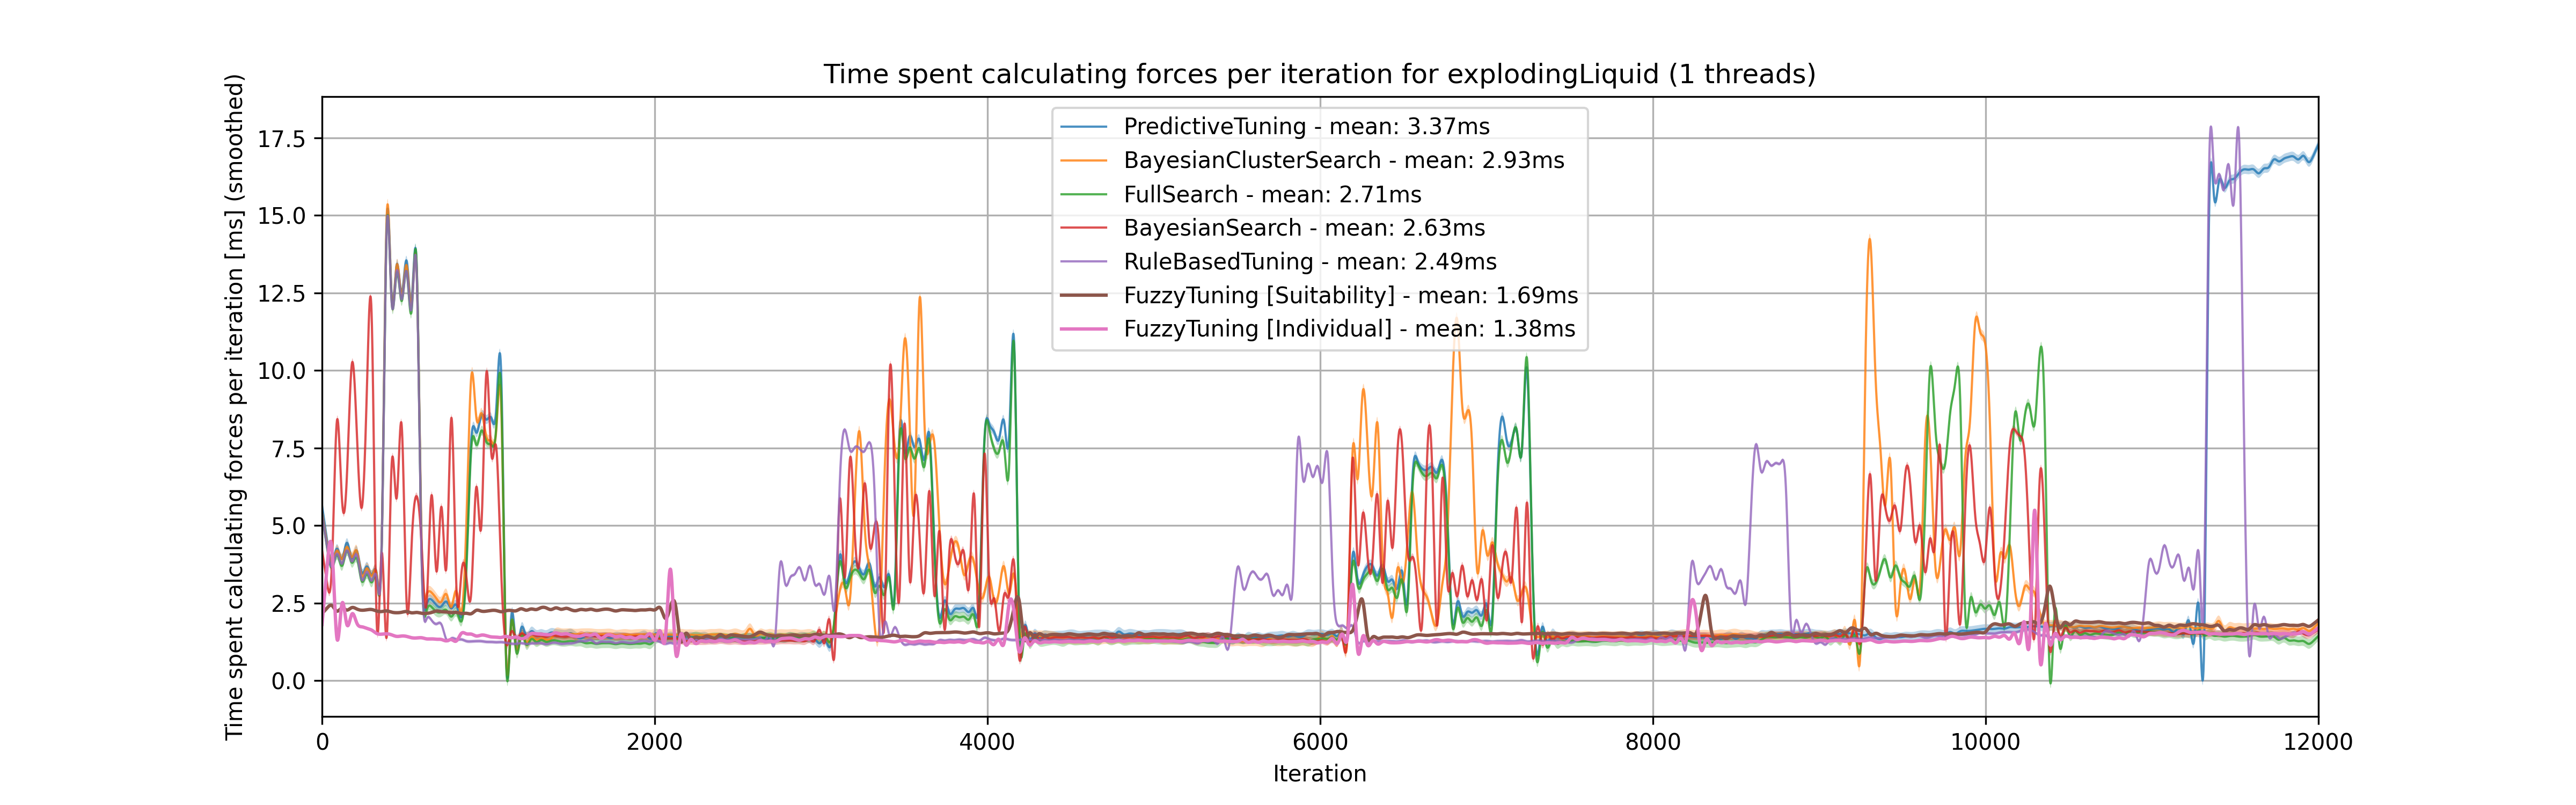
\includegraphics[width=\columnwidth,trim={1cm 0 2cm 0.5cm},clip]{figures/Benchmark/timing_explodingLiquid_1.png}
        \caption{}
        \label{fig:explodingLiquid1Benchmark_1thread}
    \end{subfigure}

    \begin{subfigure}[b]{\textwidth}
        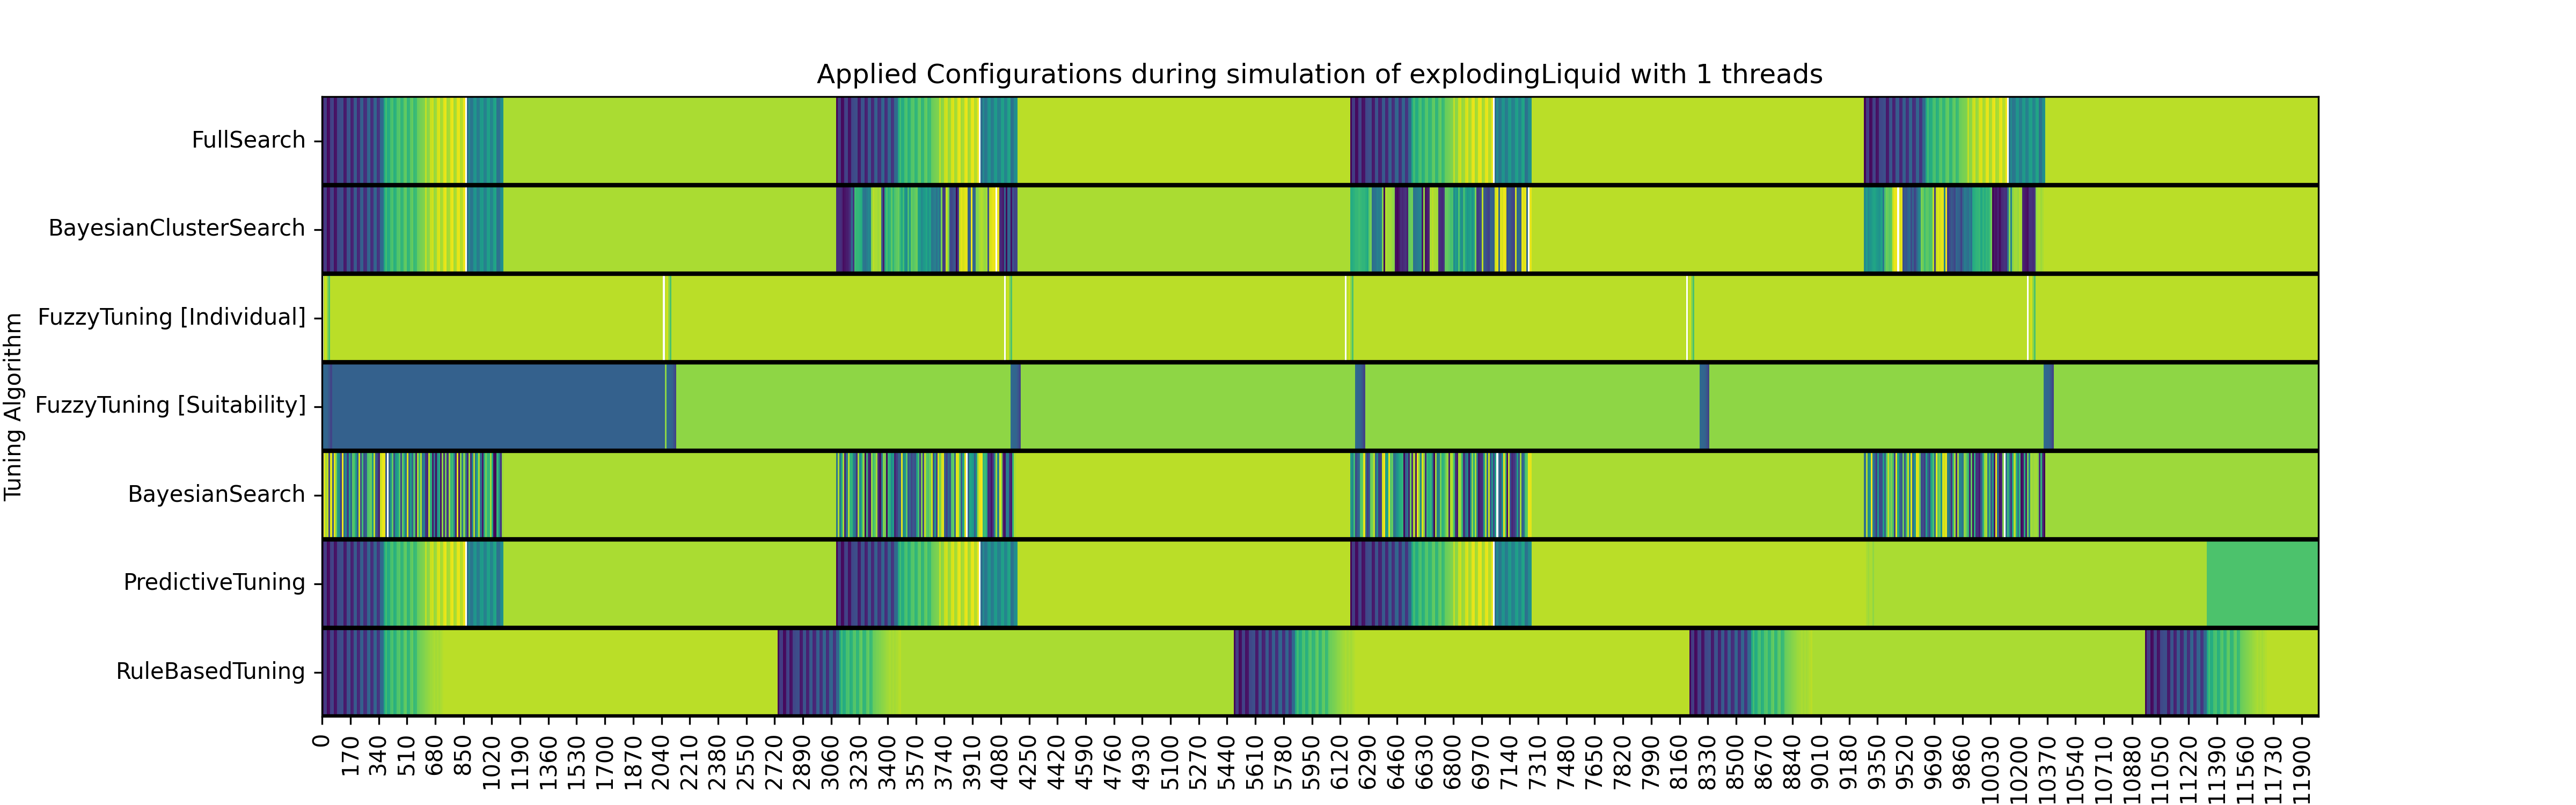
\includegraphics[width=\columnwidth,trim={0.5cm 0 0cm 0.5},clip]{figures/Benchmark/heatmap_explodingLiquid_1.png}
        \caption{}
        \label{fig:explodingLiquid1Heatmap_1thread}
    \end{subfigure}

    \begin{subfigure}[c]{\textwidth}
        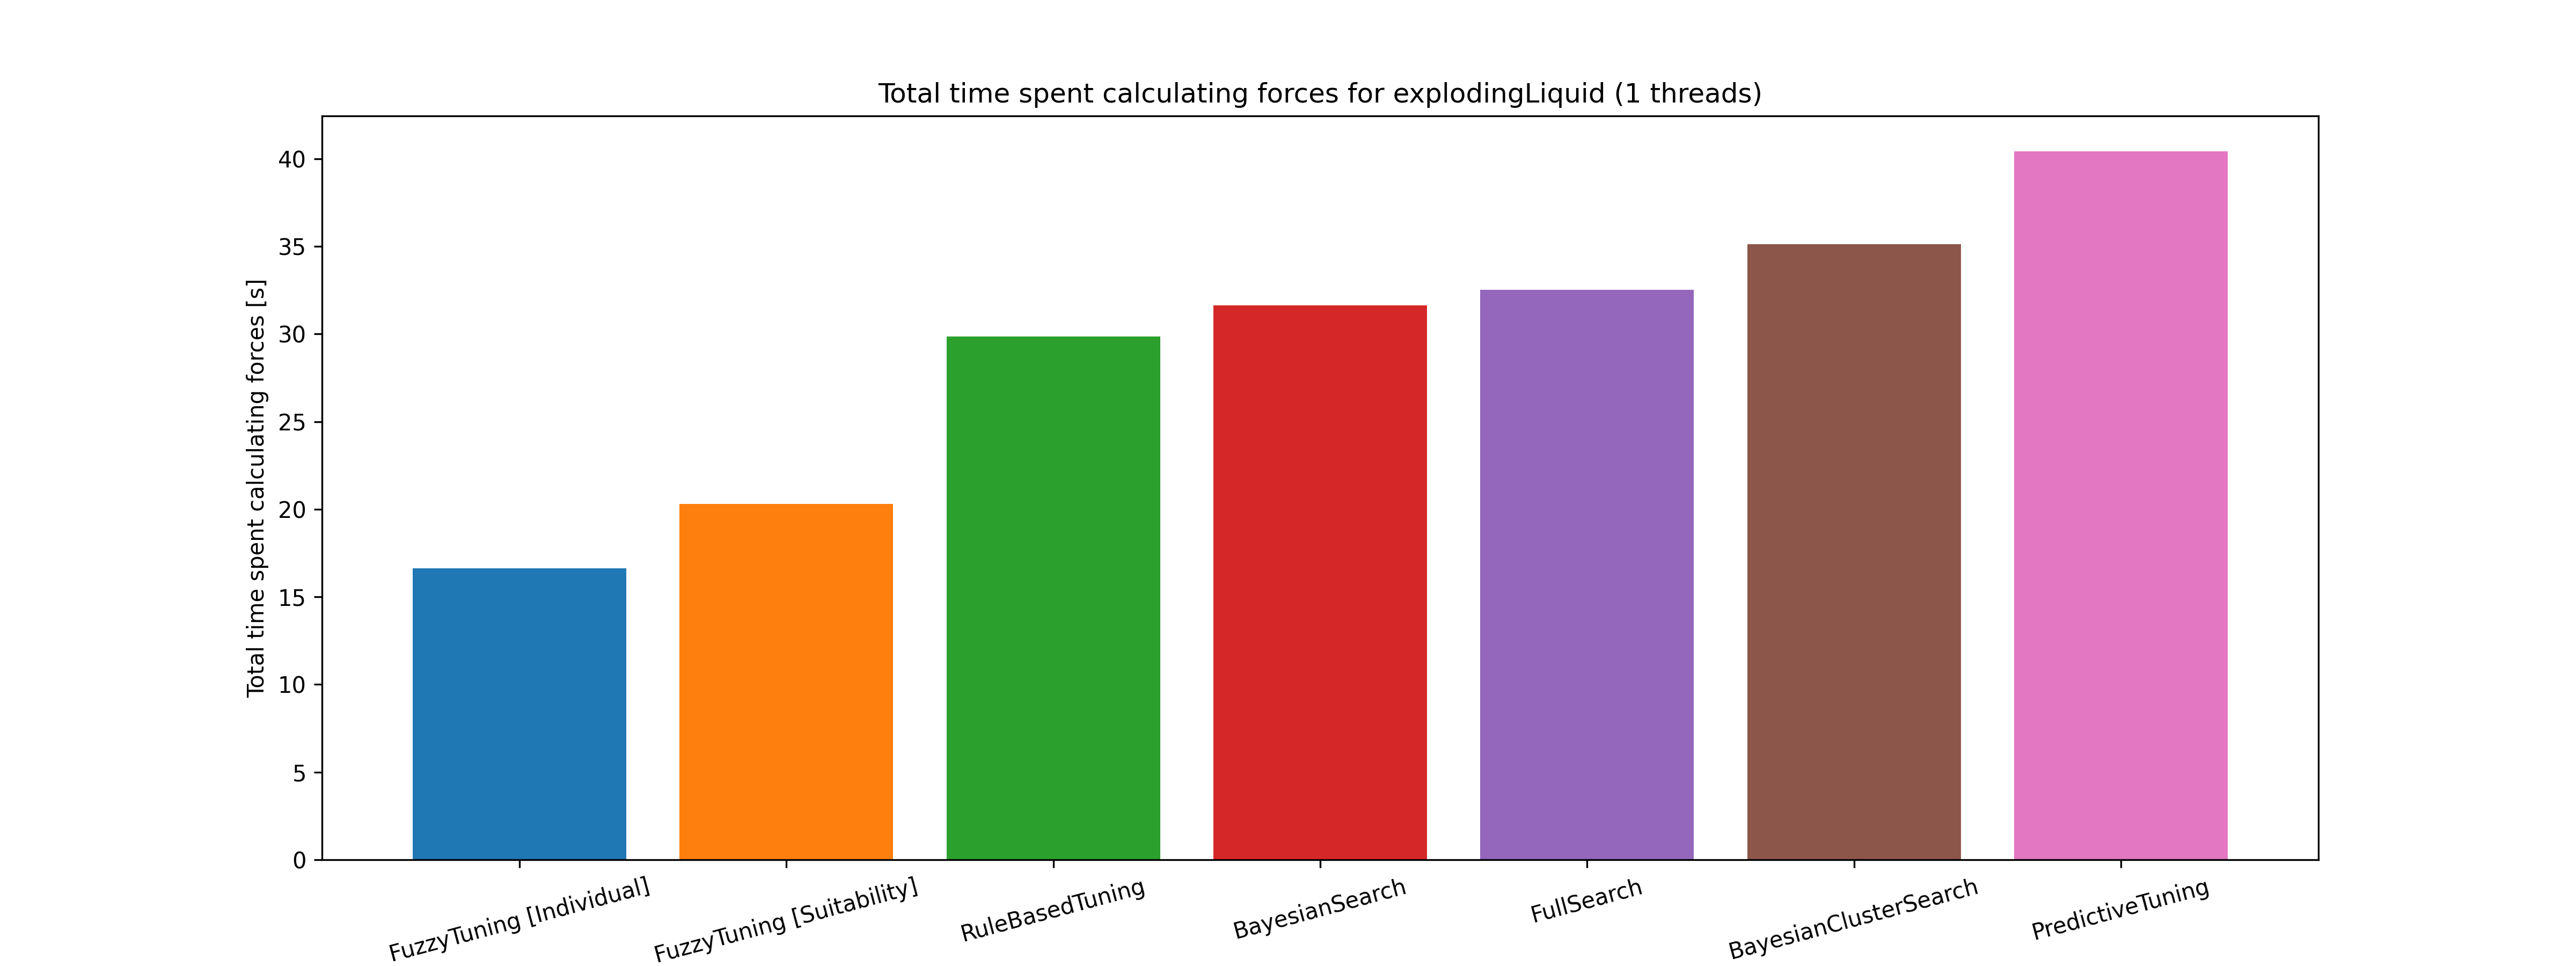
\includegraphics[width=\columnwidth,trim={0.5cm 0 0cm 0.5},clip]{figures/Benchmark/total_time_explodingLiquid_1.png}
        \caption{}
        \label{fig:explodingLiquid1TotalTime_1thread}
    \end{subfigure}

    \caption[Exploding liquid benchmark with 1 thread]{(a) Total time spent calculating the forces for the exploding liquid benchmark with 1 thread. (b) Heatmap of the tested configurations during the benchmark. The meaning of the colors are displayed in \ref{fig:colorbar_explodingLiquid}. (c) Total time spent calculating the forces for each tuning strategy.
    }

\end{figure}


\begin{figure}[H]
    \centering
    \begin{subfigure}[b]{0.94\textwidth}
        \addtolength{\leftskip} {-0.28cm} % increase (absolute) value if needed
        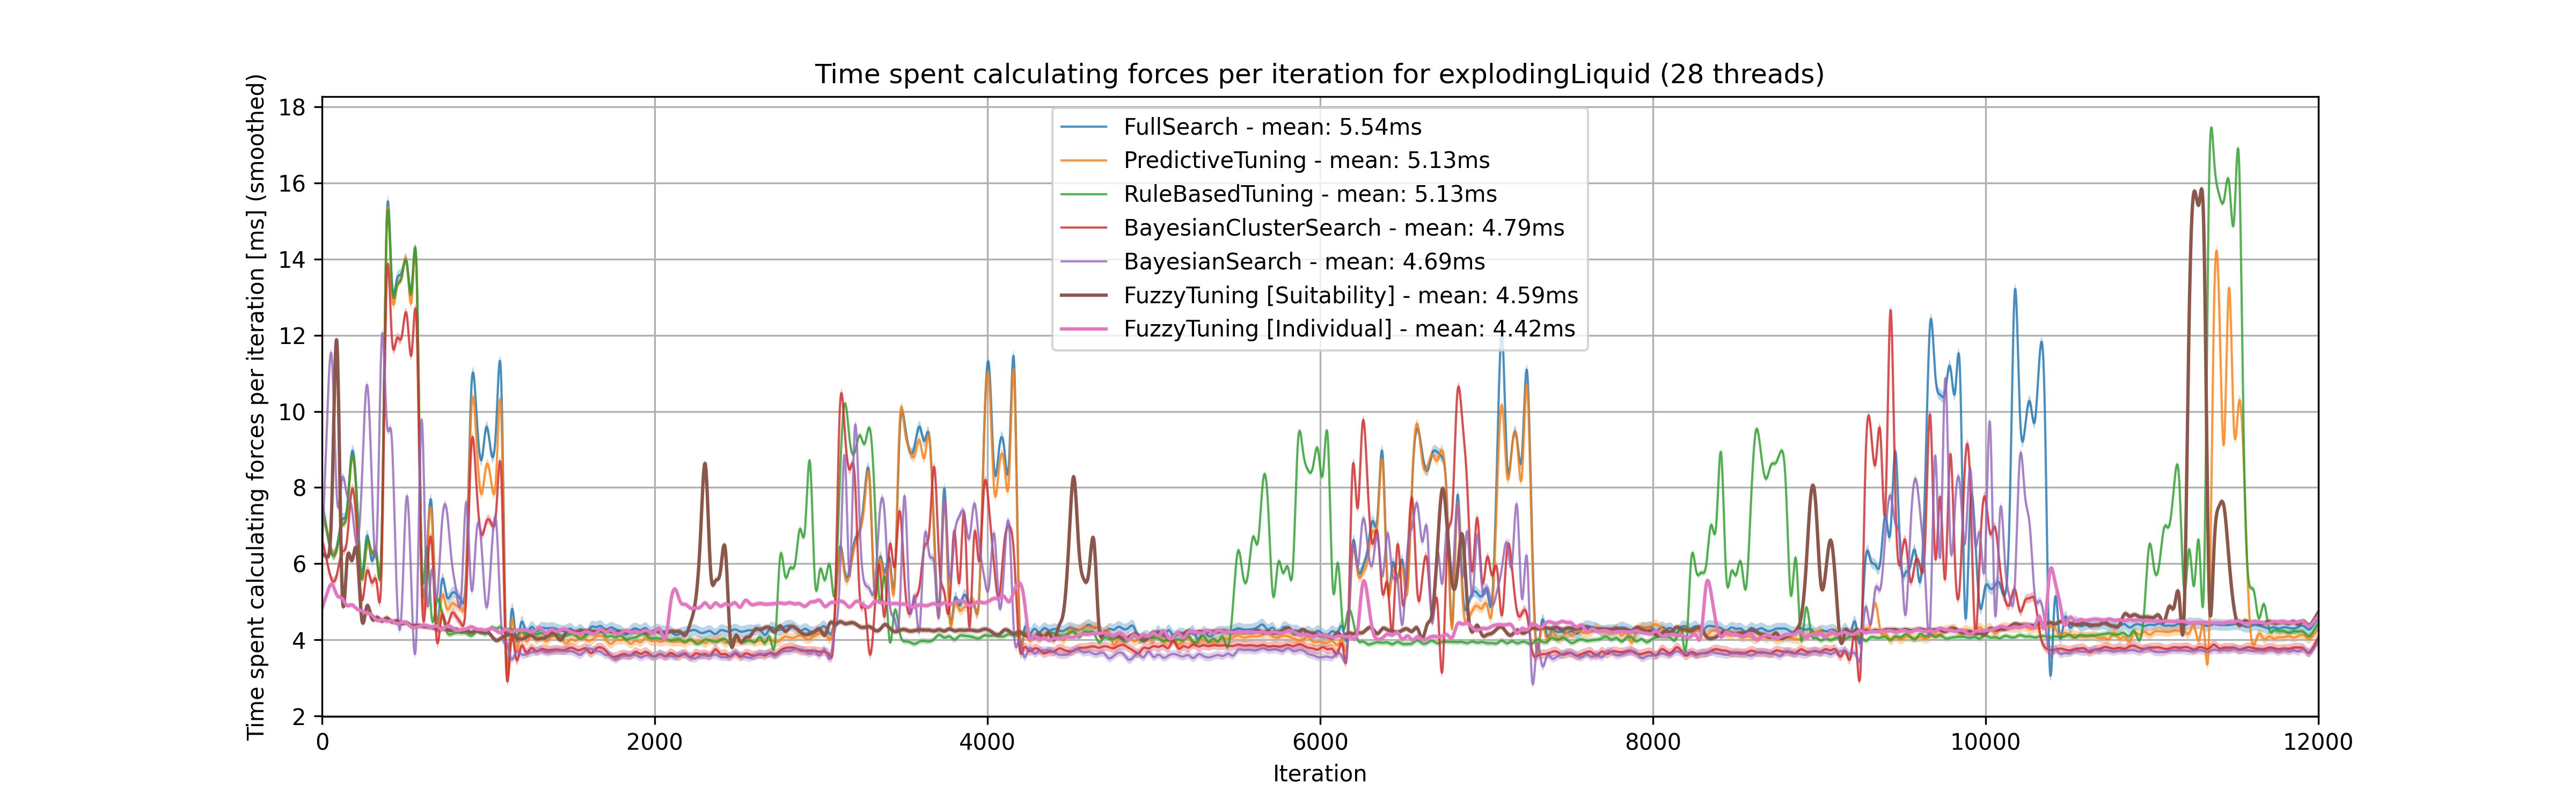
\includegraphics[width=\columnwidth,trim={1cm 0 2cm 0.5cm},clip]{figures/Benchmark/timing_explodingLiquid_28.png}
        \caption{}
        \label{fig:explodingLiquid1Benchmark_28thread}
    \end{subfigure}

    \begin{subfigure}[b]{\textwidth}
        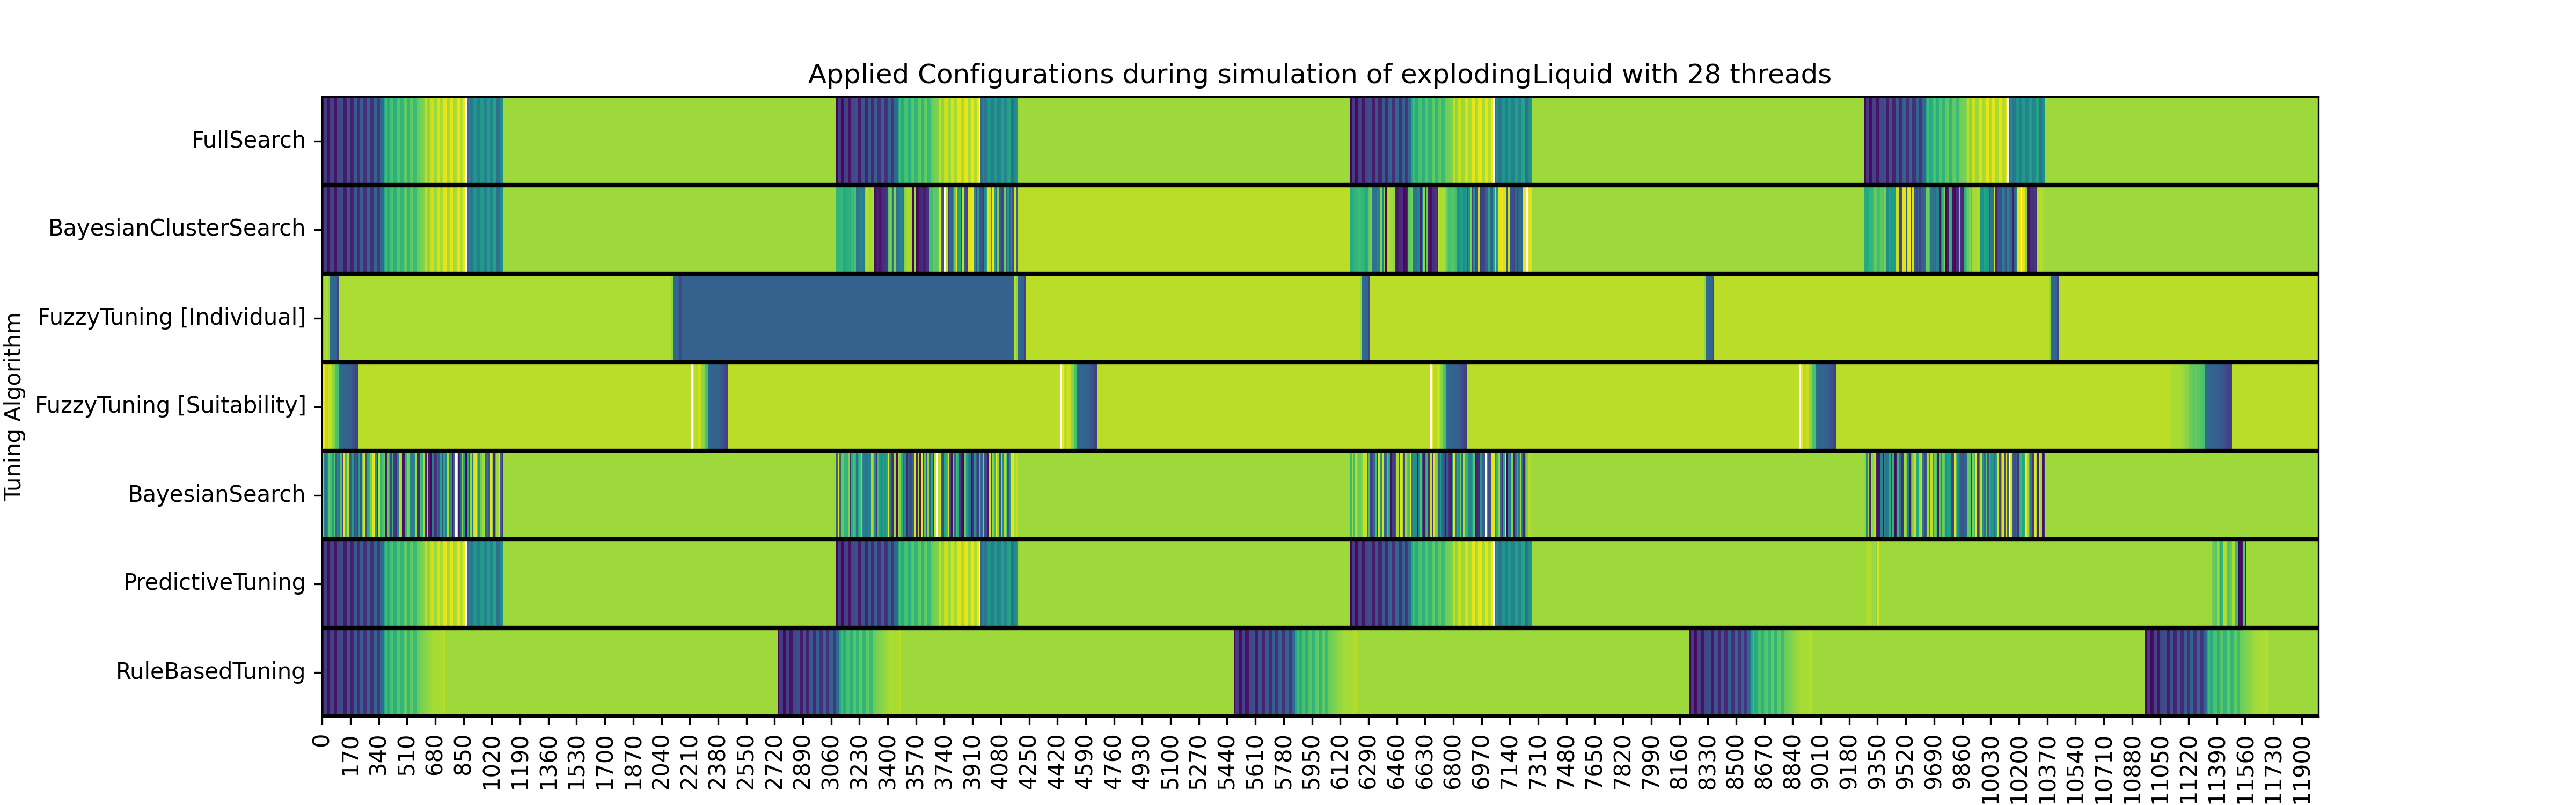
\includegraphics[width=\columnwidth,trim={0.5cm 0 0cm 0.5},clip]{figures/Benchmark/heatmap_explodingLiquid_28.png}
        \caption{}
        \label{fig:explodingLiquid1Heatmap_28thread}
    \end{subfigure}

    \begin{subfigure}[c]{\textwidth}
        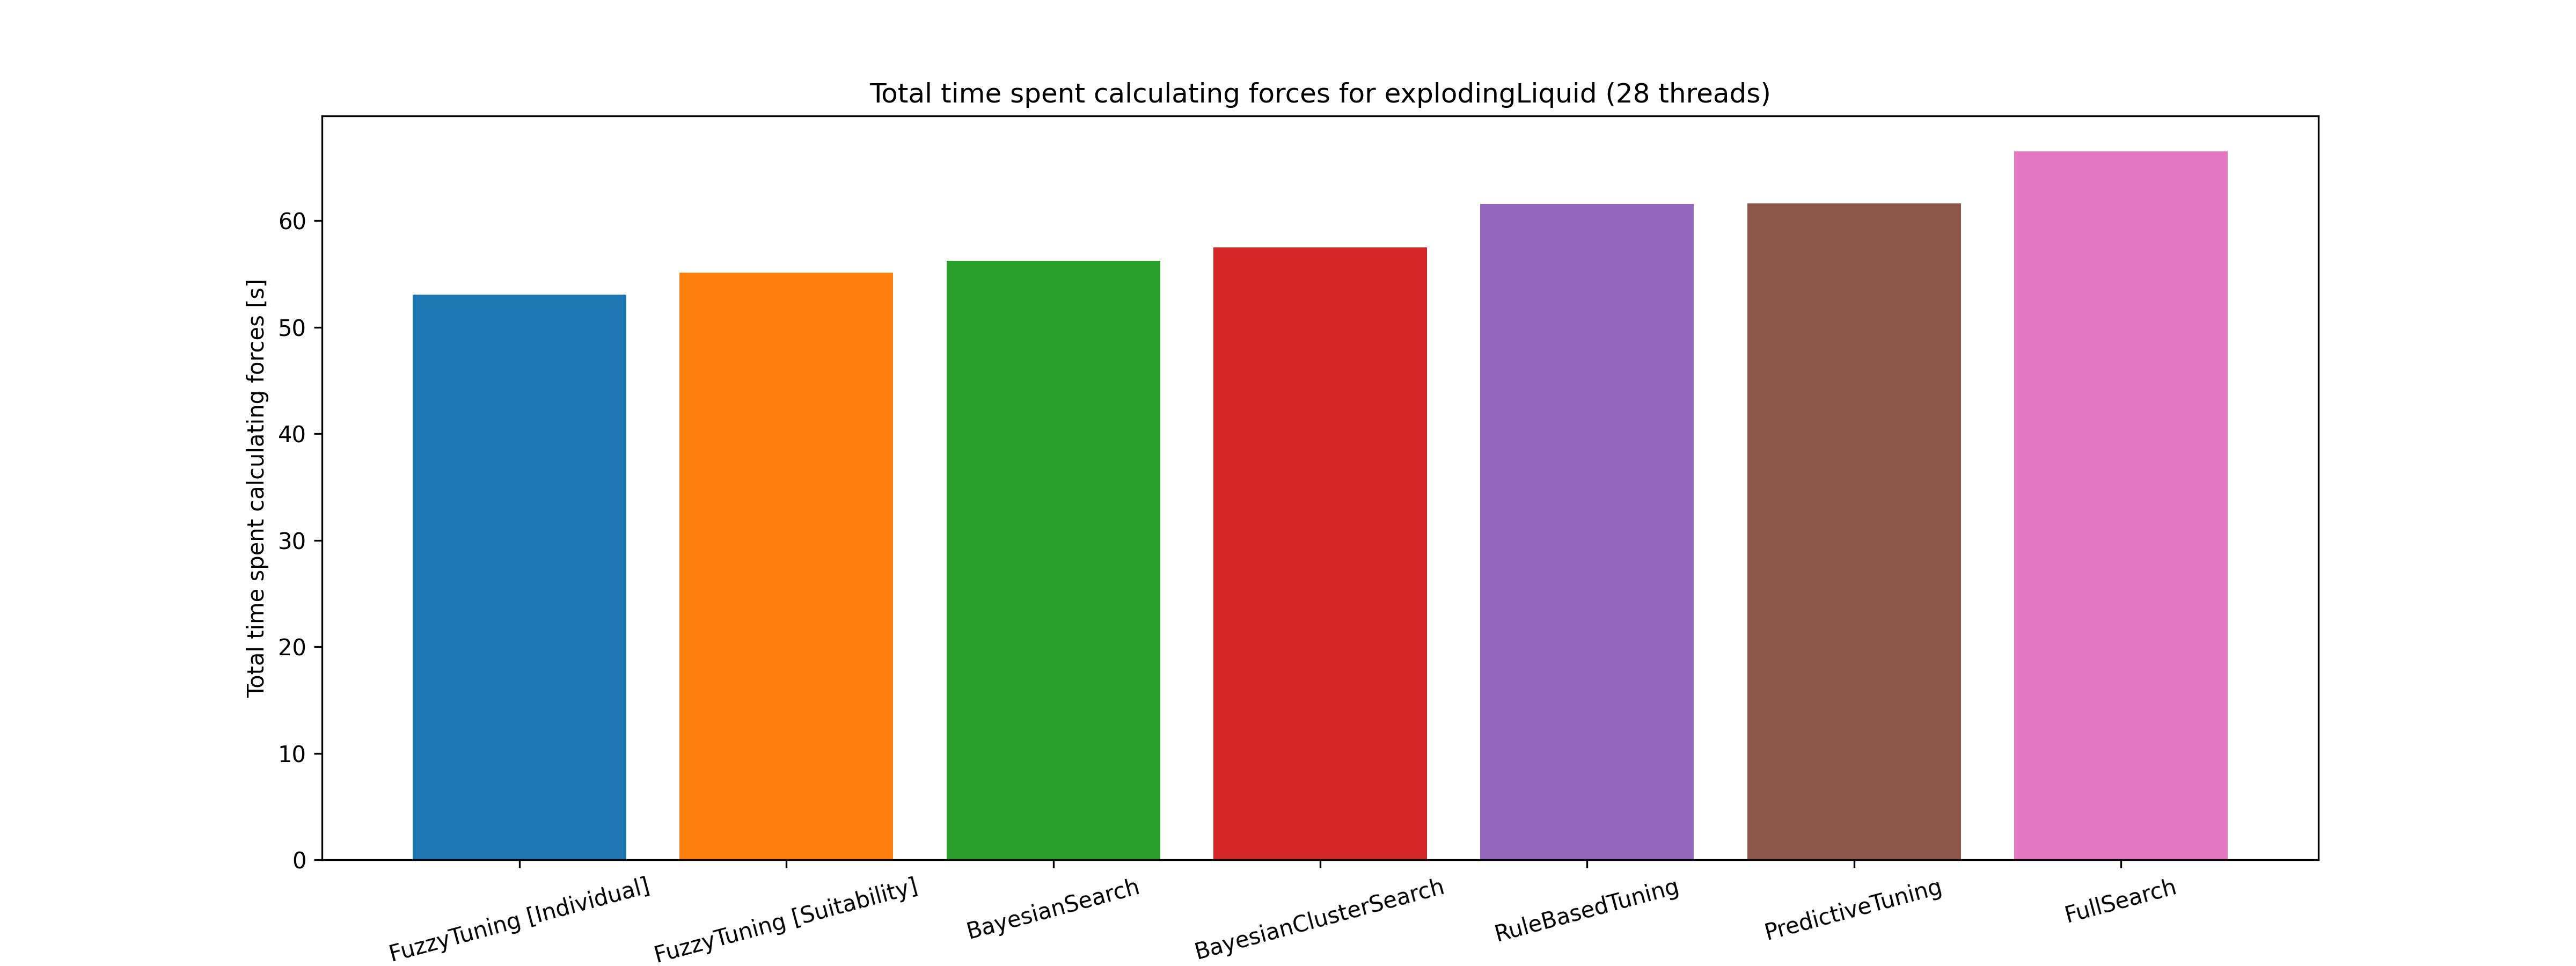
\includegraphics[width=\columnwidth,trim={0.5cm 0 0cm 0.5},clip]{figures/Benchmark/total_time_explodingLiquid_28.png}
        \caption{}
        \label{fig:explodingLiquid1TotalTime_28thread}
    \end{subfigure}


    \caption[Exploding liquid benchmark with 28 thread]{(a) Total time spent calculating the forces for the exploding liquid benchmark with 28 threads. (b) Heatmap of the tested configurations during the benchmark. The meaning of the colors are displayed in \ref{fig:colorbar_explodingLiquid}. (c) Total time spent calculating the forces for each tuning strategy.

        Note: Due to the high performance overhead of multithreading, using 28 threads results in a worse performance than using only 1 thread for this benchmark.
    }

\end{figure}





% coolmuc specs